\chapter{Top quark mass analyses in the light of full NLO calculations}
\label{chap:nlo}
%
The ever-increasing precision of \mt\ measurements requires accurate theory predictions, beyond the simplifying assumption that production and decay of a \tquark\ pair can be treated as independent.
%
In particular, this factorisation approximation neglects Feynman graphs connecting the initial and the final state. This is the basis for the \gls{NWA}, working in the zero-decay-width limit $\Gt\to0$, which additionally requires the absence of connecting elements between both \tquark\ decays. The heuristic equivalent for this is the assumption of an average lifetime large enough for production and decay to be separated. 
%
This is challenged already at \gls{NLO} precision, where a gluon can connect initial and final state or \tquark\ decay products. 
%
Moreover, the \tquark\ is one of the most short lived particles of the \gls{SM} with an average lifetime of $\tau_\mathrm{top} \approx 0.5 \cdot 10^{-24}$~s, resulting in a broad width of $\Gt\approx1.4$~\GeV~\cite{PDG2014}. 
%
Consequently, non-negligible effects due to the finite width and non-factorising contributions are expected. 
%
% In fact the fractional uncertainty on \ttbar\ production cross section calculations is observed to be $O(\Gamma_\mathrm{top}/\mt) \approx 0.9\%$ and up to $10\%$ in high \pt\ regions in the presence of phase space restrictions.\todo{add citation, update numbers!}
%
The calculation of the full process \ppWWbb\ naturally takes into account non-factorising contributions and includes resonant, singly resonant and non-resonant contributions of \tquark\ production and decay.

This chapter presents an investigation of the numerical impact of the full \gls{NLO} calculation and its related uncertainties compared to the commonly used \gls{NWA} approach in the framework of \mt\ measurements. The study is performed at \genlevel. It is the result of a collaboration of groups from phenomenological and experimental physics and published in \reference~\cite{Heinrich2014}. 


%
% Unlike previous investigations~\cite{Biswas:2010sa}, non-factorising contributions are taken into account for the first time.















\section{Status of Monte Carlo modelling}
%
The last decades have seen a dramatic improvement of the \tquark\ pair production modelling, ranging from the \gls{NLO} \gls{QCD} corrections~\cite{Nason:1987xz,Beenakker:1990maa,Frixione:1995fj} over the \gls{NLO} \gls{EW} corrections~\cite{Beenakker:1993yr} to the \gls{NNLO} calculation, which has only recently become available~\cite{Czakon:2013goa,Top2015NNLOtopxsec}.
%
Today's standard \gls{MC} generator programs employ the aforementioned \gls{NWA} for the \tquark\ pair decay modelling, still mostly at \gls{LO}, preserving spin correlations via techniques like spin density matrices or reweighting. 
%
Further improvement has been achieved by a \gls{NLO} treatment of \tquark\ pair decays and a consistent evaluation of production and decay including spin correlations at \gls{NLO}, using the \gls{NWA}~\cite{Melnikov:2009dn,Biswas:2010sa,Melnikov:2011ai}. However, this is still limited to \genlevel. 



A consistent treatment of \tquark\ pair production and decay at \gls{NLO} without any factorisation assumption necessarily leads to the inclusion of terms without a \ttbar\ intermediate state. These can be divided into singly resonant or non-resonant contributions, depending on the number of \tquark\ propagators in the corresponding Feynman diagram that can be on the mass shell, i.e. satisfying the relation $E^2=p^2+m^2$, as shown in \fig~\ref{fig:resonant}. Without factorisation, the process \ppttbarWWbb\ becomes \ppWWbb, summing up all intermediate states and treating the \tquark{s} as off-shell particles. This comes with a significant rise in complexity, because the process to be calculated is no longer a $2 \to 2$ process with the decay treated separately, but a $2 \to 4$ process, connecting the incoming protons with the final state. This calculation is not only desirable because of its consistency in higher order perturbation theory, but it is also closer to reality, where singly and non-resonant contributions constitute irreducible physics background. Consequently, their consistent treatment in the calculation provides a more accurate description of the experimentally accessible final state.
%
%%%%%%%%%%%%%%%%%%%%%%%%%%%%%%%%%%%%%%%%%%%%%%%%%%%%%%%%%%%%%%%%%%%%%%%%%%%%%%%
\begin{figure*}[tbp!]
\centering
\subfloat[Resonant term]{
  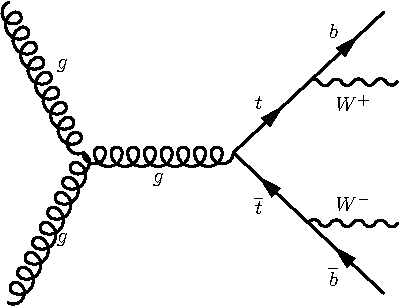
\includegraphics[width=0.3\textwidth]{./figs/resonant.pdf}
  \label{sfig:resonant}
}
\subfloat[Singly resonant term]{
  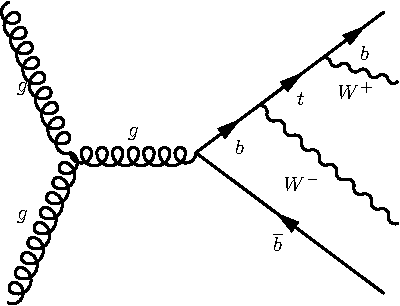
\includegraphics[width=0.3\textwidth]{./figs/sresonant.pdf}
  \label{sfig:sresonant}
}
\subfloat[Non-resonant term]{
  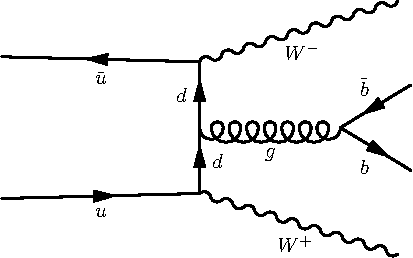
\includegraphics[width=0.3\textwidth]{./figs/nonresonant.pdf}
  \label{sfig:nonresonant}
}  
\caption[Terms in a \ppWWbb\ calculation]{
%
Representative tree-level Feynman diagrams illustrating the resonant~\subref{sfig:resonant}, singly resonant~\subref{sfig:sresonant} and non-resonant~\subref{sfig:nonresonant} terms present in the calculation of the \ppWWbb\ process.
%
This and all subsequent figures are published in \reference~\cite{Heinrich2014}.
%
\label{fig:resonant}
}
\end{figure*}
%%%%%%%%%%%%%%%%%%%%%%%%%%%%%%%%%%%%%%%%%%%%%%%%%%%%%%%%%%%%%%%%%%%%%%%%%%%%%%%
%
After a pioneering full calculation of the process \ppWWbb\ at \gls{NLO} using massless \bquark{s} (5-flavour scheme), but ignoring the contribution of initial state \bquark{s}~\cite{Denner:2010jp,Denner:2012yc,Bevilacqua:2010qb}, a calculation including massive \bquark{s} (4-flavour scheme) has been achieved~\cite{Frederix:2013gra,Cascioli:2013wga}.
















\section{Calculational framework}
%
The work presented in the following is based on the calculation documented in \reference~\cite{Heinrich2014}. 
%
It employs a computation in the 5-flavour scheme of the $\order(\alphas^2\alpha^2)$ process $pp\to W^+W^-b\bar{b}\to$\newline$(e^+ \nu_e)\,(\mu^- \bar{\nu}_{\mu})\,b\bar{b}$ with \gls{NLO} \gls{QCD} corrections, including initial state \bquark\ contributions. 
%
Diagrams involving Higgs bosons are neglected, just as non-resonant \Wboson\ and \Zboson\ contributions, whose impact has been found to be small~\cite{Denner:2012yc}. 
%
% The sub-process involving $b\bar b$ in the initial state is generated separately from the other quark--anti-quark annihilation processes, because the \bquark{s} may propagate to the final state, which adds additional diagrams.
% separately 
%
The large number of Feynman diagrams necessitates automatic diagram generation and algebraic manipulation~\cite{Nogueira:1991ex,Vermaseren:2000nd, Reiter:2009ts, Cullen:2010jv}, which is provided by the one-loop amplitude package \Gosam~\cite{Cullen:2011ac}. 
%
% It is linked via the Binoth--Les-Houches interface~\cite{Binoth:2010xt,Alioli:2013nda} to the multi-purpose \gls{MC} event generator \Sherpa~\cite{Gleisberg:2008ta}, which provides the Born, real radiation and subtraction term contributions and performs the phase-space integration.
%
\Tquark\ width effects are taken into account by employing the complex mass scheme~\cite{Denner:2006ic}, which preserves gauge invariance. 
%
% This can be accomplished by replacing \mt\ in the calculations with the complex number $\mu_\mathrm{top}^2\;=\;\mt^2-i\;\!\mt\Gamma_\mathrm{top}$. 
%
%The neglection of \Wboson\ and \Zboson\ contributions leaves the weak mixing angle real-valued.
%
% The strong coupling constant \alphas\ and its running are set according to the MSTW2008 \gls{LO} and \gls{NLO} parton distributions~\cite{MAR-0901}. 
%
The \tquark\ mass is set to $\mt=172.5$~\GeV\ and the \pp\ collision \cme\ to $\sqrts=7$~\TeV.
%
The other quarks are treated as massless. 
%
% The \tquark\ decay width is set to $\Gamma_\mathrm{top}^\mathrm{(N)LO}=1.4426 (1.3167)$~\GeV~\cite{Jezabek:1988iv}.
%
%Giorgio says this is too detailed:
% Besides that, the following \gls{EW} paramers in the $G_{\mu}$ scheme\todo{What is the $G_{\mu}$ scheme?} are used:
% %
% \begin{equation*}
%   \begin{matrix}
%    G_{\mu} &=& ~1.16637\cdot10^{-5}&\GeV^{-2},~~& \\[1mm]
%    m_{W}  &=& 80.399~\GeV\,,\hphantom{0}     && \Gamma_W &=& 2.0997~\GeV\,,\\
%    m_{Z}  &=& 91.1876~\GeV\,,                && \Gamma_Z &=& 2.5097~\GeV\,.
%   \end{matrix}
% \end{equation*}
%
Results obtained with this setup have been compared to previous calculations in selected phase space regions and found to be consistent within uncertainties~\cite{Denner:2012yc}.
%



To assess the effects of the finite width treatment in the simulation of the \ttbar\ process, calculations of the $(e^+ \nu_e)\,(\mu^- \bar{\nu}_{\mu})\,b\bar{b}$ final states using two different setups were performed. 
%
In the full approach, the $2\to4$ process \ppWWbb\ is calculated at \gls{LO} or \gls{NLO} precision, fully taking into account finite width effects of the \tquark{s} and non-resonant contributions. 
%
In the factorised approach, the $2\to2$ process \ppttbar\ is calculated at \gls{NLO} precision, while the \ttbar\ decay is evaluated at \gls{LO} precision, based on the \gls{NWA}. This approach is referred to as narrow width approximation with leading-order decays.
%
As detailed in \reference~\cite{Heinrich2014}, contributions neglected in the \gls{NWA} are suppressed by powers of $\Gt/\mt\lesssim1\%$. However, this holds for cross section calculations and sufficiently inclusive variables, while the impact on variables like the estimator \mlb, making use of only some of the physical final states, may be different. 
%
In the following, the differences of the full and the factorised approach at \genlevel\ applied in a direct \tquark\ mass measurement are investigated.






\section{Phase space and object definition}
%
The phase space and physics objects have been defined as closely as possible to the experimental setup of the $\sqrts=7$~\TeV\ analysis, described in \chap~\ref{chap:topmass7TeV}.
%
%%%%%%%%%%%%%%%%%%%%%%%%%%%%%%%%%% merged selection %%%%%%%%%%%%%%%%%%%%%%%%%%%%%%%
\Genlevel\ jets are constructed from final state partons using the \antikt\ jet clustering algorithm~\cite{CAC-0801} implemented in \Fastjet~\cite{Cacciari:2011ma} with an $R$ parameter of $0.4$ and a spatial jet separation requirement of $\dR_\mathrm{jj}>0.4$. At least two \bjet{s} with $\pt>25~\GeV$\ and $\abseta<2.5$ are required, which are defined as jets containing a \bquark\ among the clustered particles. 
%
Electrons are required to have $\pt>25~\GeV$ and muons to have $\pt>20~\GeV$. All leptons have to satisfy $\abseta<2.5$. Since the generated final state is the e$^+\mu^-$ decay channel, the restrictions on the number of electrons and their flavour and charge are met by default. 
%
A spatial separation of jets and leptons of $\dR_\mathrm{l,j}>0.4$ is required.
%
% The \met\ is defined as the transverse vector sum of the two neutrinos and required to be $\met>20$~\GeV. \\not used in emu channel!
%
The \Ht\ variable is defined as $\Ht=\sum_i {\pt}_{,i}$ with the sum running over all final state particles, including neutrinos. An \Ht\ requirement reflecting the experimental conditions is applied by defining $\Ht^\mathrm{exp}$ as the sum over the transverse momenta of leptons, excluding neutrinos, and jets and requiring $\Ht^\mathrm{exp}>130$~\GeV.
%
The default renormalisation and factorisation scales are chosen as $\mur=\muf=\mu\equiv \Ht/2$. This choice is motivated by the relative stability against scale variations and the small difference of the \gls{LO} and \gls{NLO} results for the resulting cross sections.
%
The corresponding inclusive \gls{LO} and \gls{NLO} cross sections for the full approach in the above defined phase-space are 
%
\[
\begin{aligned}
  \sigma_{\gls{LO}} &\;=\; 638.4\,^{+38.5\%}_{-24.8\%}\,(\text{scale})\;\pm\;0.03\%\,(\text{stat})~\fb,\\[1mm]
  \sigma_{\gls{NLO}} &\;=\; 758.5\,^{-2.5\%}_{-5.3\%}\,(\text{scale})\;\pm\;0.2\%\,(\text{stat})~\fb,
\end{aligned}
\]
%
corresponding to a ratio of about $1.2$ of the \gls{NLO} to the \gls{LO} inclusive cross sections (\kfac). The scale uncertainties have been evaluated from a variation of the central scale $\mu$ by a factor of 2 and 1/2, corresponding to $x=1/2$ and $x=2$ with $x=\frac{\mu}{\Ht/2}$. As shown in \fig~\subref*{sfig:scale}, the \gls{NLO} cross section at the central scale is close to a maximum. Consequently, both scale variation uncertainties are negative. 
%
%The statistical uncertainties stem from the \gls{MC} integration process. 
%
\Fig~\subref*{sfig:pTbmax} shows the differential cross section as a function of the leading \bjet\ \pt\ at \gls{LO} and \gls{NLO}. The bands indicate the scale variation uncertainty. A comparison of the size of the uncertainty bands shows the drastically reduced uncertainty at \gls{NLO} and also the harder \pt\ spectrum, stemming from the possibility of a gluon radiation recoil against the \ttbar\ system. The \gls{LO} prediction is coated by a flat uncertainty band, while the \gls{NLO} band depends on \pt. 
%
In contrast to global uncertainties like the one of the total cross section, phase space dependent uncertainties are relevant for the shape sensitive analysis used in the \tquark\ mass measurements.
%
%%%%%%%%%%%%%%%%%%%%%%%%%%%%%%%%%%%%%%%%%%%%%%%%%%%%%%%%%%%%%%%%%%%%%%%%%%%%%%%
\begin{figure*}[tbp!]
\centering
\subfloat[Total \ttbar\ production cross section]{
  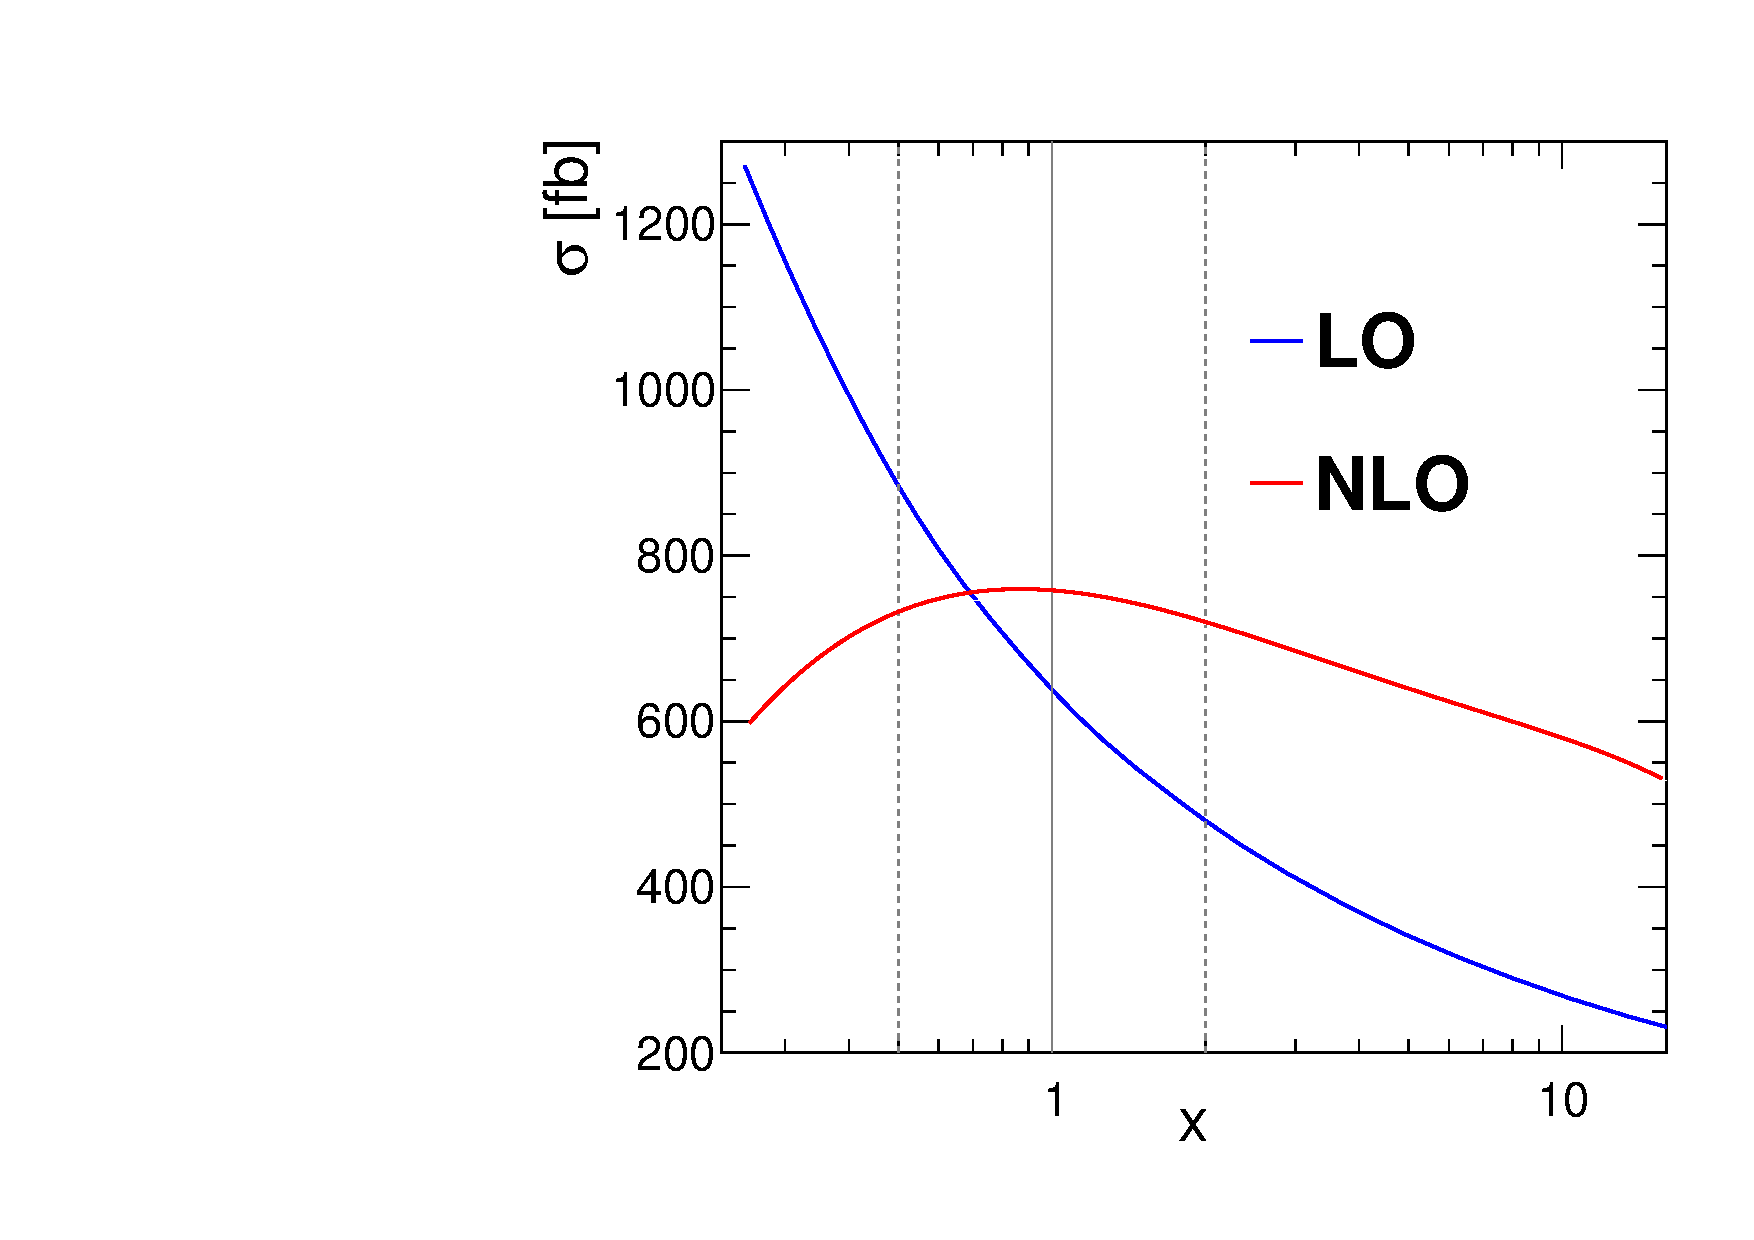
\includegraphics[width=0.49\textwidth]{./figs/scalevar.pdf}
  \label{sfig:scale}
}
\subfloat[Leading \bjet\ \pt\ distribution]{
  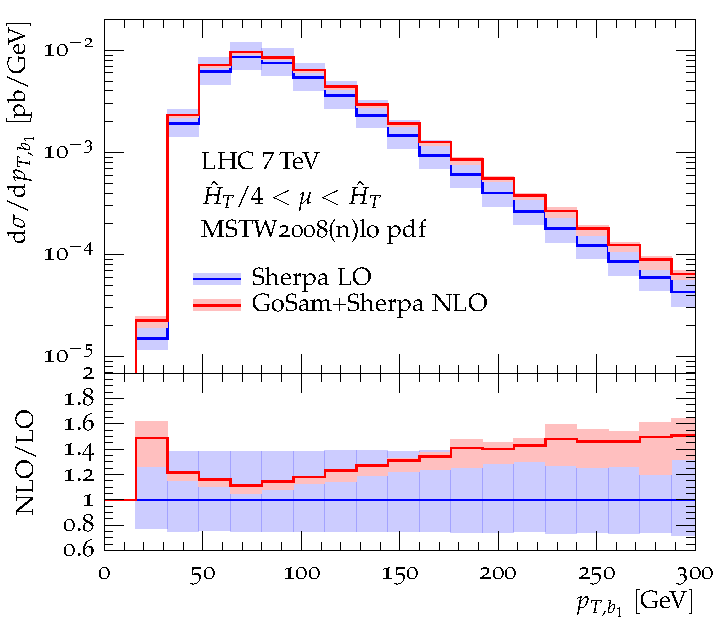
\includegraphics[width=0.49\textwidth]{./figs/pTbmax.pdf}
  \label{sfig:pTbmax}
}
\caption[Effects of scale variation]{
%
\gls{LO} and \gls{NLO} cross section results \subref{sfig:scale} in the full approach as a function of the central scale $\mu$ in the range $x=\frac{\mu}{\Ht/2}=1/4...16$, with the chosen central scale at $x=1$.
%
The leading \bjet\ \pt\ distribution \subref{sfig:pTbmax} at \gls{LO} and \gls{NLO} with uncertainty bands corresponding to a scale variation of a factor of 2 and 1/2 around $\mu=\Ht/2$~\cite{Heinrich2014}.
%
}
\label{fig:scalevar}
\end{figure*}
%%%%%%%%%%%%%%%%%%%%%%%%%%%%%%%%%%%%%%%%%%%%%%%%%%%%%%%%%%%%%%%%%%%%%%%%%%%%%%%
%















\section[Effects on the \texorpdfstring{\mlb}{mlb} estimator distribution]{Effects on the \texorpdfstring{\boldmath$\mlb$}{mlb} estimator distribution}
%
\Tquark\ measurements rely on \mt\ dependent differential distributions. Consequently, they are affected by shape altering modelling uncertainties, like a variation of the renormalisation and factorisation scales $\mur$ and $\muf$. 
%
At \recolevel, the corresponding effect on \mt, obtained from present \gls{MC} models, is relatively small, compared to other modelling uncertainties. The impact of these variations at \genlevel\ on a measurement, similar to the \dil\ measurements presented in this work, is investigated in the following.

To follow the experimental approach as closely as possible, the \mlb\ variable is taken as estimator and constructed the same way as detailed in \sect~\ref{sect:dilreco7TeV}. 
%
The resulting differential cross sections as functions of \mlb\ are shown in \fig~\subref*{sfig:mlbfull} for the full and in \fig~\subref{sfig:mlbnwa} for the factorised approach at \gls{LO} and \gls{NLO} precision, with the uncertainty band covering the scale variations. 
%
Here and in all following figures, the full (factorised) approach is denoted by \WWbbplusminus\ (\ttbar).
%
The scale choice for the full approach is the standard dynamic choice $\mu=\Ht/2$, while for the factorised approach it is fixed to $\mu=\mt$. 
%
The \gls{NLO} predictions lie within the uncertainty bands of the \gls{LO} predictions, except for the tails. Here, the full calculation predictions differ significantly and also, in the factorised approach, the last bins before the \gls{LO} kinematic cut-off at $\mlb > \sqrt{\mt^2-\mW^2} \approx 150$~\GeV\ hint at the same feature. This kinematic cut-off for the factorised approach is a consequence of the fact that at \gls{LO} both \bquark--lepton systems stem from an on-shell \tquark. 
%
The \gls{LO} tail in the full calculation is a result of the events that are added to the signal by the inclusion of the non-resonant terms. At \gls{NLO}, it is even more pronounced.
%
 % by misreconstruction in presence of \gls{NLO} radiation.
%
The uncertainty bands of the factorised calculation are larger than the ones of the full calculation. In contrast to the full approach, the \gls{NLO} relative corrections using the factorised approach are flat in the bulk region. Similarly, the scale variation uncertainty bands are centred around the mean value, while for the \gls{NLO} full approach they are not. Consequently, in the factorised approach, the \gls{NLO} and scale variation effects mainly change the event rate, while in the full approach they affect the shape of the observable distribution as well. 
%
Consistent results have been found using the fixed scale for the full approach, so the difference is not dominated by the scale choice.
%
%%%%%%%%%%%%%%%%%%%%%%%%%%%%%%%%%%%%%%%%%%%%%%%%%%%%%%%%%%%%%%%%%%%%%%%%%%%%%%%
\begin{figure*}[tbp!]
\centering
\subfloat[\gls{LO} vs \gls{NLO} for the full calculation]{
  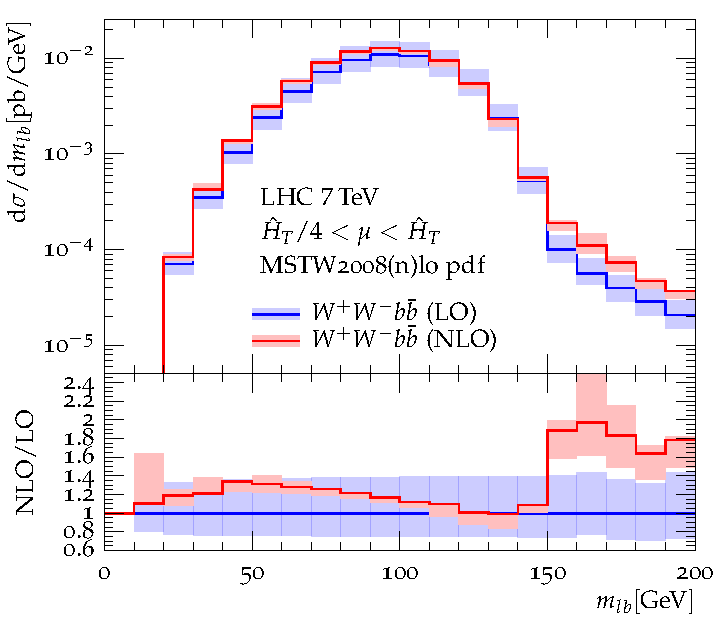
\includegraphics[width=0.49\textwidth]{./figs/mlb_scalevar_wwbb.pdf}
  \label{sfig:mlbfull}
}
\subfloat[\gls{LO} vs \gls{NLO} for the factorised calculation]{
  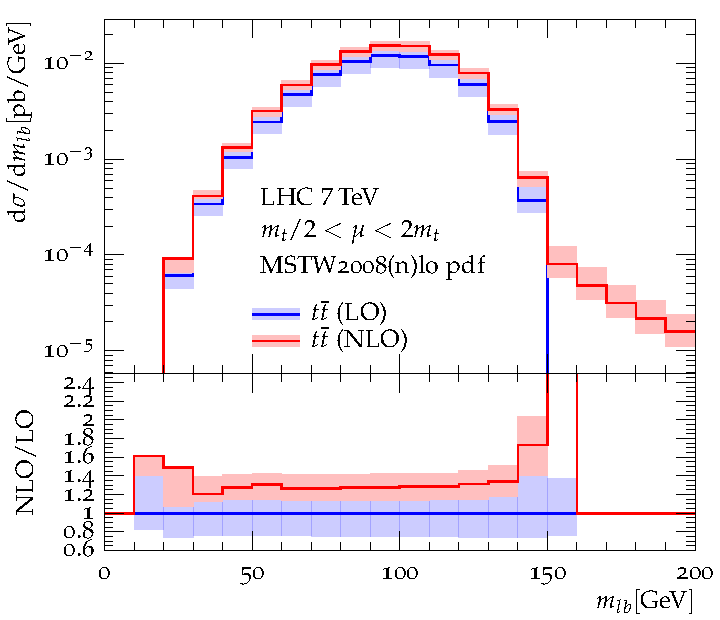
\includegraphics[width=0.49\textwidth]{./figs/mlb_scalevar_tt.pdf}
  \label{sfig:mlbnwa}
}
\\
\subfloat[Full and factorised calculation]{
  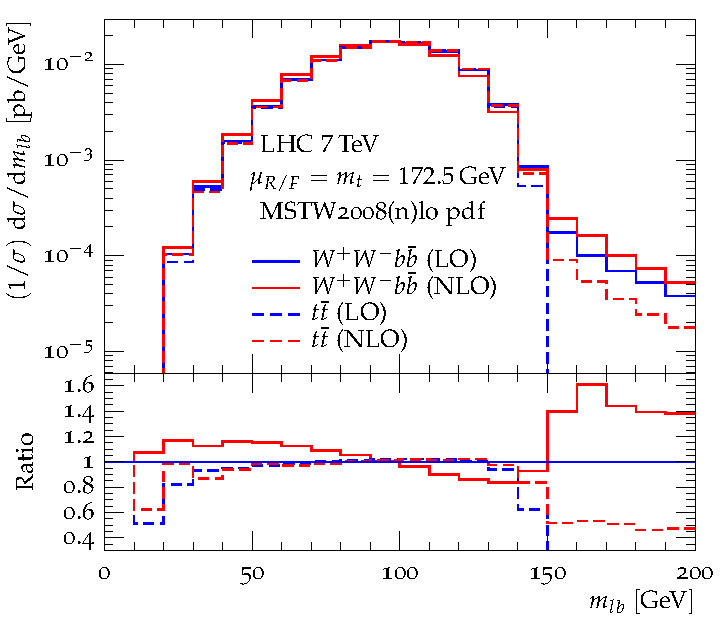
\includegraphics[width=0.49\textwidth]{./figs/mlb_compare_tt_wwbb.pdf}
  \label{sfig:mlbcalc}
}
\subfloat[\mt\ dependence of full calculation]{
  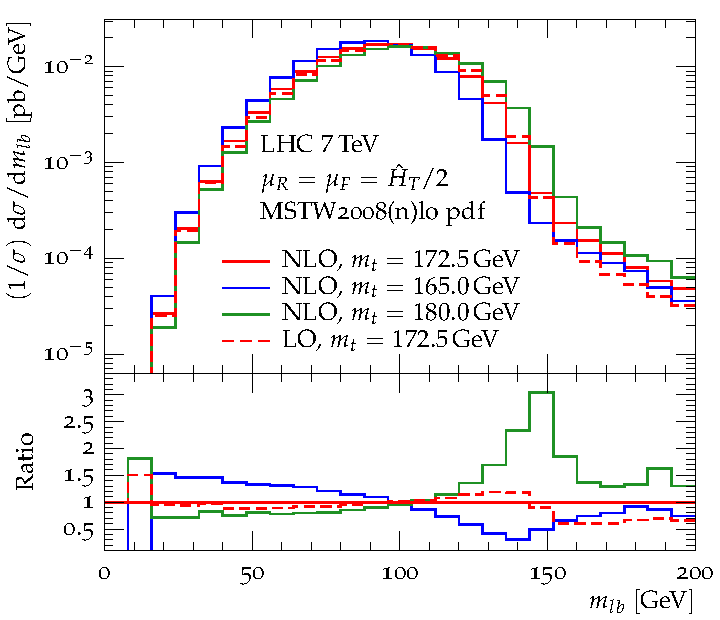
\includegraphics[width=0.49\textwidth]{./figs/mlb_norm0_log1_NLOLO.pdf}
  \label{sfig:mlbmass}
}
\caption[\mlb\ distributions at \gls{NLO}]{
%
Differential cross sections as functions of \mlb\ for~\subref{sfig:mlbfull} the full and~\subref{sfig:mlbnwa} the factorised approach at \gls{LO} and \gls{NLO} precision, with the uncertainty band corresponding to the standard scale variations. The scale choice for the full approach is dynamic ($\mu=\Ht/2$), while for the factorised approach it is fixed ($\mu=\mt$). The \gls{LO} result is taken as reference in the ratio shown below. 
%
In \fig~\subref{sfig:mlbcalc}, the full and factorised calculations are compared using a fixed scale. The \gls{LO} full calculation approach is used as reference in the ratio shown below.
%
In \fig{s}~\subref{sfig:mlbfull} to \subref{sfig:mlbcalc}, the distributions are shown for $\mt=172.5$~\GeV, and \gls{LO} distributions are drawn in blue, \gls{NLO} distributions in red. 
%
\Fig~\subref{sfig:mlbmass} shows the dependence of the full \gls{NLO} \mlb\ distributions on the input \mt\ value. For comparison, the $\mt=172.5$~\GeV\ prediction at \gls{LO} (dashed line) is drawn as well.
}
\label{fig:mlbnlo}
\end{figure*}
%%%%%%%%%%%%%%%%%%%%%%%%%%%%%%%%%%%%%%%%%%%%%%%%%%%%%%%%%%%%%%%%%%%%%%%%%%%%%%%
%

A comparison of distribution shapes is most relevant for the \mt\ measurement, and this is displayed at \gls{LO} and \gls{NLO} in \fig~\subref*{sfig:mlbcalc} for the full and factorised approach. Since the calculations are reasonably stable with respect to the scale choice, the technically more convenient fixed scale $\mu=\mt$ is used in the factorised approach. The distributions are normalised and depicted without uncertainty bands. Apart from the aforementioned differences in the tail, a considerable \mlb\ dependent deviation of the full \gls{NLO} prediction from the other distributions of up to $20\%$ in the bulk is visible. This can lead to a potentially large difference in the measured \mt.
%
\Fig~\subref*{sfig:mlbmass} shows the effect of a changed \mt\ parameter on the distributions, where \mt\ can be identified with the \tquark\ pole mass. Here, \mlb\ distributions calculated with the full approach are displayed for several \mt\ values at \gls{NLO}. The experimental measurements are based on the sensitivity of the \mlb\ variable to \mt, whose effect is visible in the ratio histograms. 
%
Judging from the observed differences in \fig{s}~\subref{sfig:mlbcalc} and \subref{sfig:mlbmass}, an impact of non-factorising effects of $\order(\GeV)$ can be expected.
%$20\%/60\%\cdot 7.5~\GeV=2.5~\GeV$ from non-factorising effects can be expected.




















\section{Effects on \tquark\ mass measurements}
%
Using the \genlevel\ predictions of the \mlb\ distributions for different values of \mt\ as templates, a template method similar to the ones described in \chap{s}~\ref{chap:topmass7TeV} and \ref{chap:topmass8TeV} is set up. 
%
Templates are constructed from the cross sections differential in \mlb, and a $\chi^2$ fit is used to determine the \mt\ parameter. This fit can then be used to quantify the difference of any pair of \mlb\ distributions in terms of \mt\ at \genlevel. 
%
Following the analysis presented in \chap~\ref{chap:topmass7TeV}, 1000 pseudo-datasets according to $\intlumi=4.7~\invfb$ are drawn from the \gls{NLO} prediction at $\mt=172.5$~\GeV\ and $\sqrts=7$~\TeV\ and analysed with a template fit function corresponding to either the \gls{LO} or the \gls{NLO} model. 
%
The data are represented in this case by the best available prediction. This mimics the situation of analysing experimental data with template fit functions calibrated to templates from a given model, which may be different. 
%
Due to the sizeable differences in the predicted distribution shape, separate fit functions are used for the factorised and the full approach and the effects are evaluated separately. A showcase pseudo-experiment is given for each, the factorised approach in \fig~\subref*{sfig:pseudott} and the full approach in \fig~\subref{sfig:pseudoWWbb}, together with the respective fitted template fit functions in red. 
%
The prediction, according to which the pseudo-dataset is drawn, is displayed as black histogram. In both cases the fitted \mt\ value \mtout\ is consistent within uncertainties with the input value $\mtin=172.5$~\GeV. 
%
% The mean values of the distributions differ by almost $2~\GeV$ and also the predicted cross section, the normalisation of the distributions, is higher in the factorised approach by about $20\%$. 
%
% This is another sign of the sizeable differences of the factorised and the full approach. 

%
%%%%%%%%%%%%%%%%%%%%%%%%%%%%%%%%%%%%%%%%%%%%%%%%%%%%%%%%%%%%%%%%%%%%%%%%%%%%%%%
\begin{figure*}[tbp!]
\centering
\subfloat[Factorised]{
  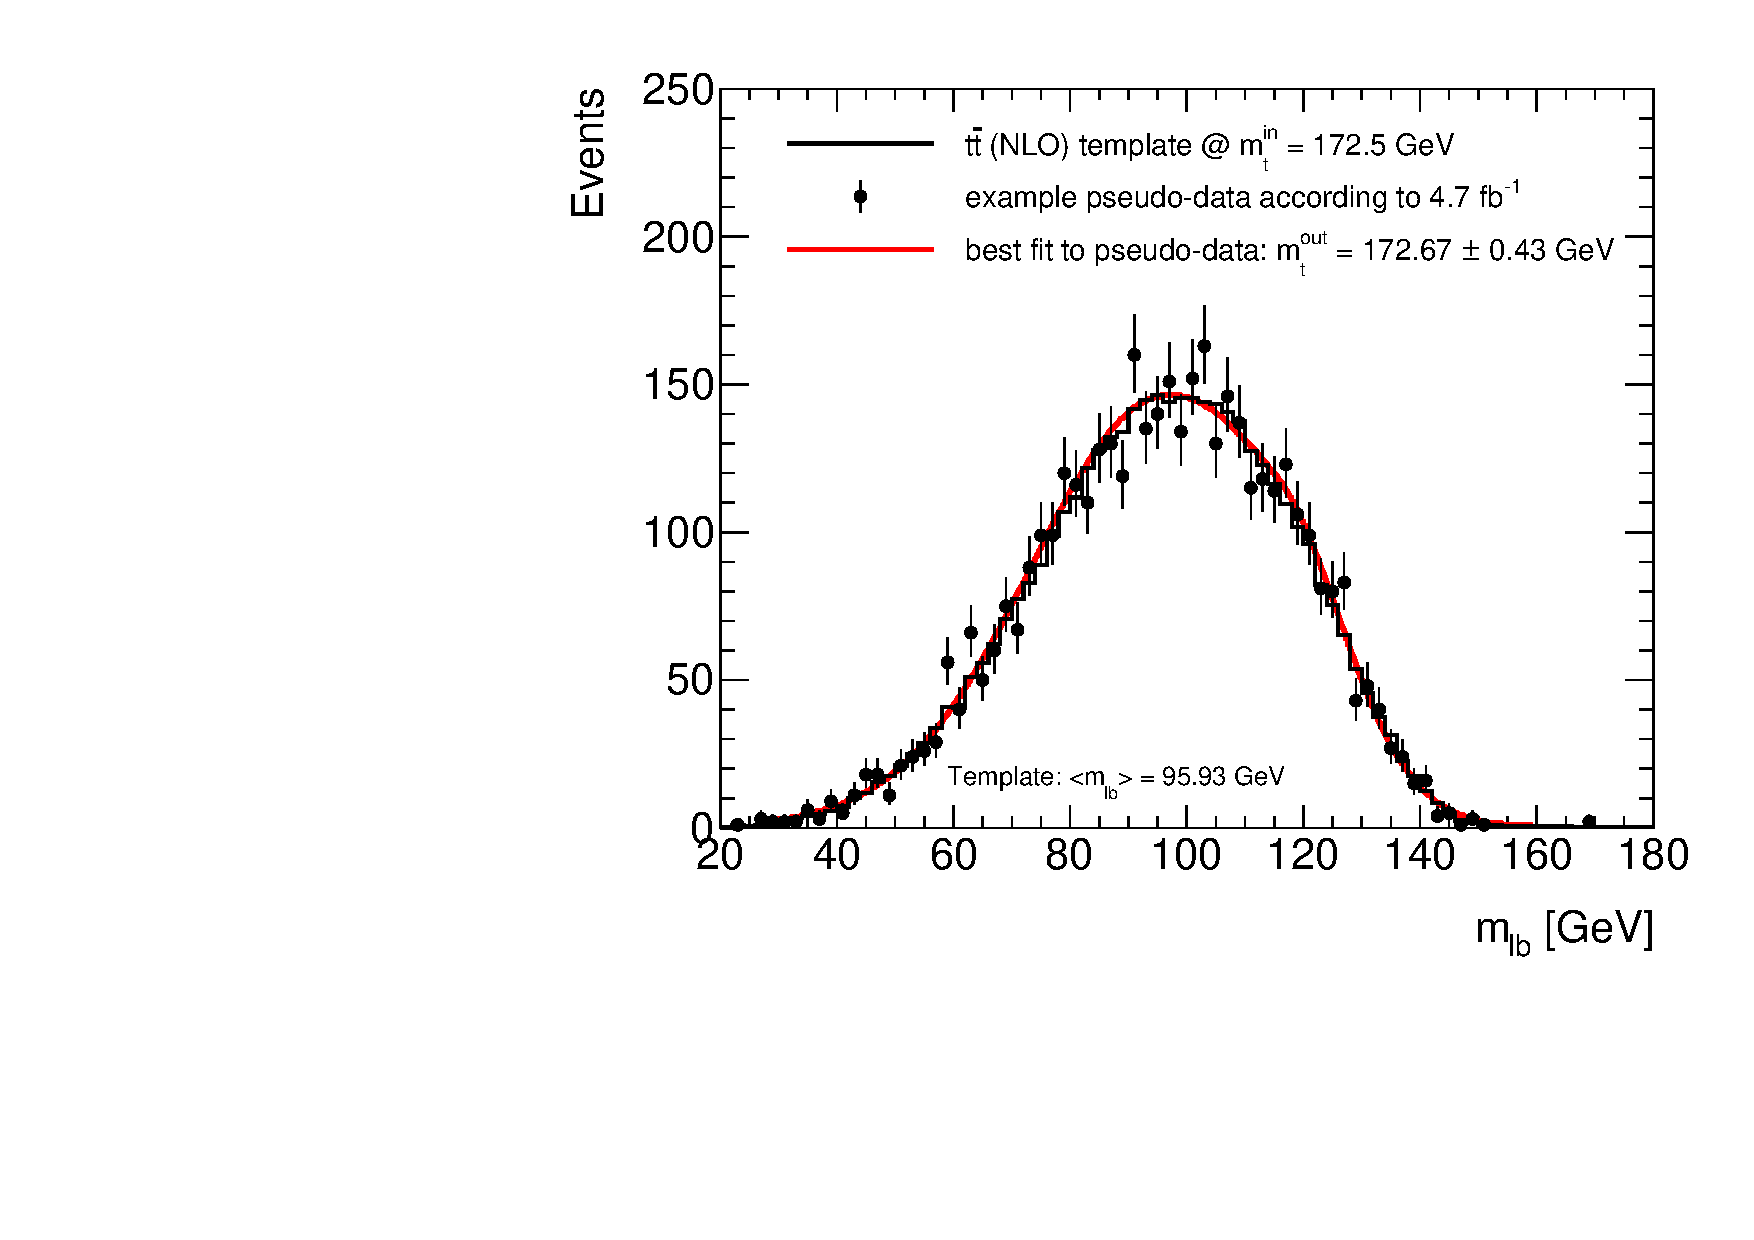
\includegraphics[width=0.49\textwidth]{./figs/fig10a.pdf}
  \label{sfig:pseudott}
}
\subfloat[Full]{
  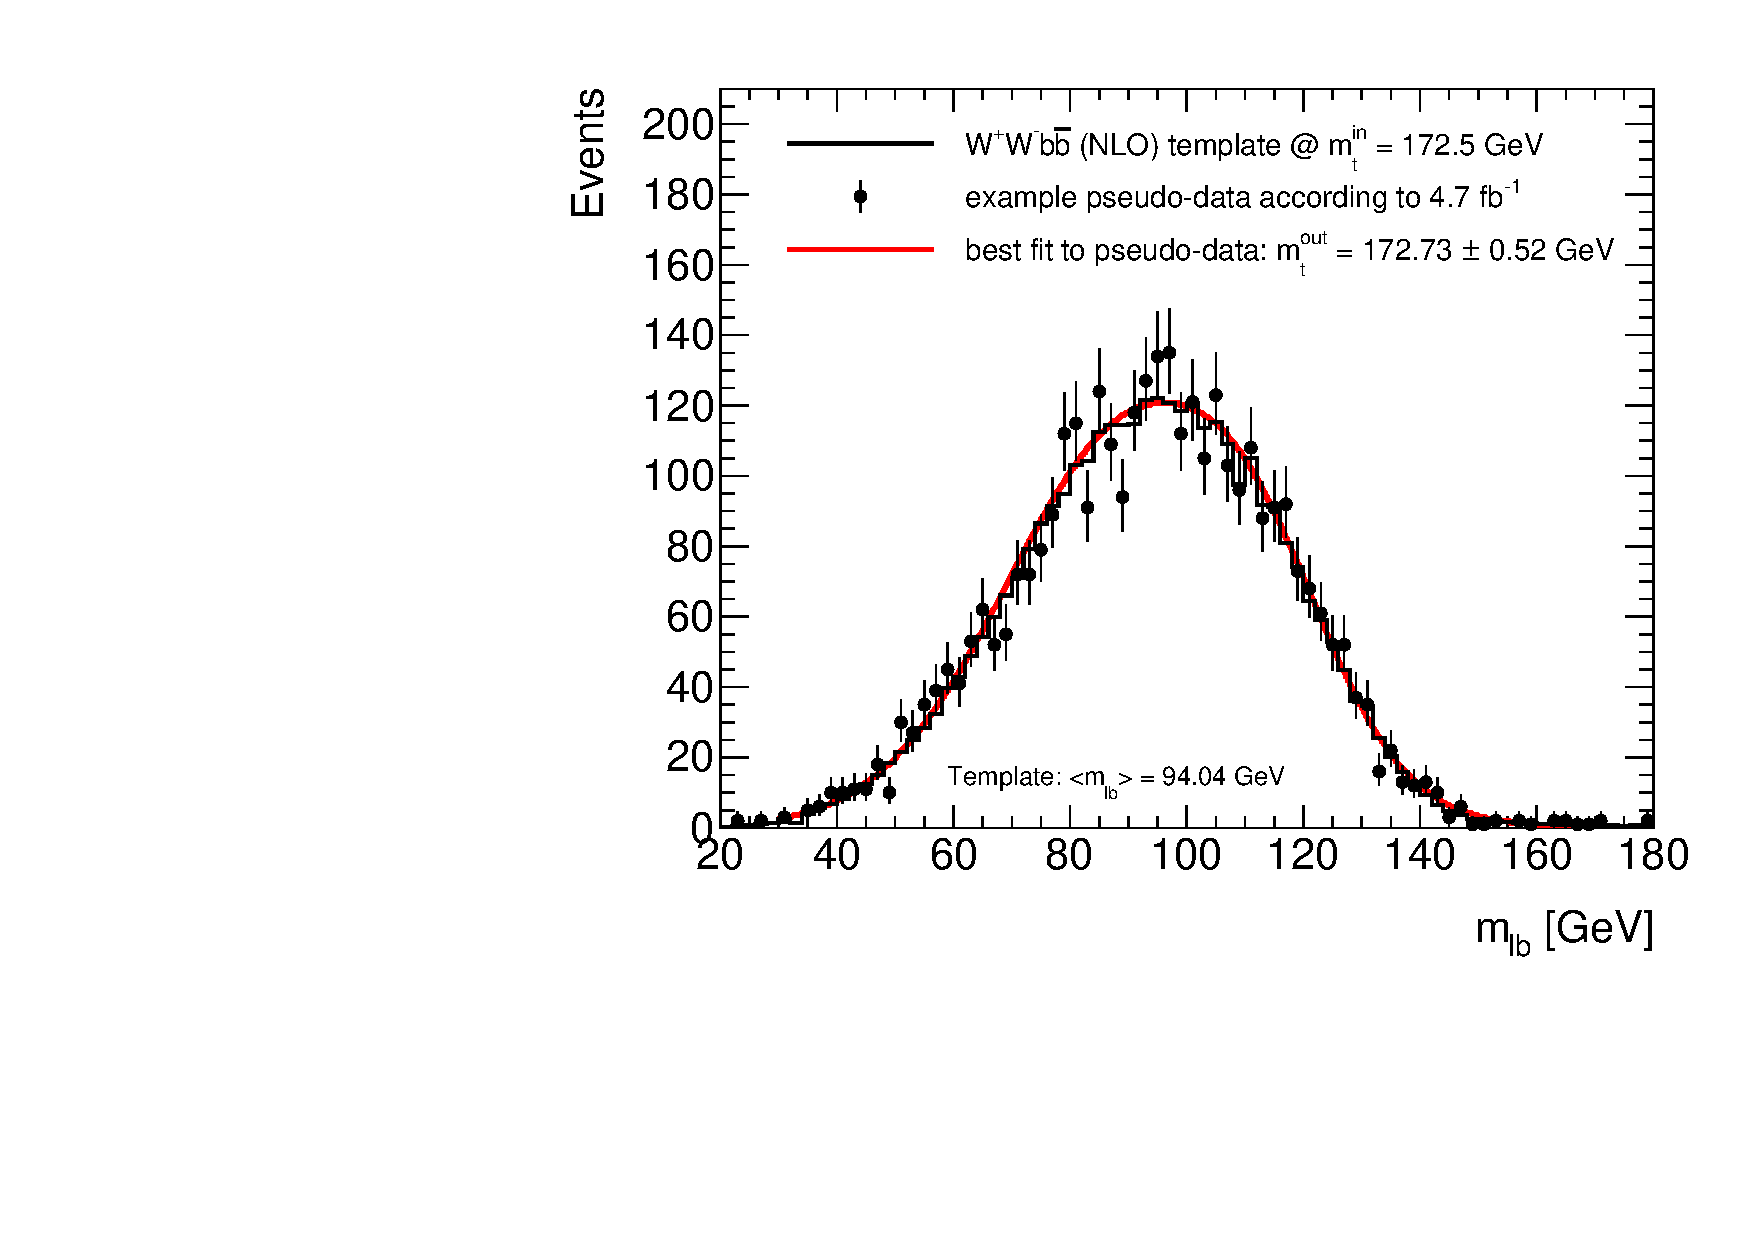
\includegraphics[width=0.49\textwidth]{./figs/fig9a.pdf}
  \label{sfig:pseudoWWbb}
}
\\
\subfloat[Factorised]{
  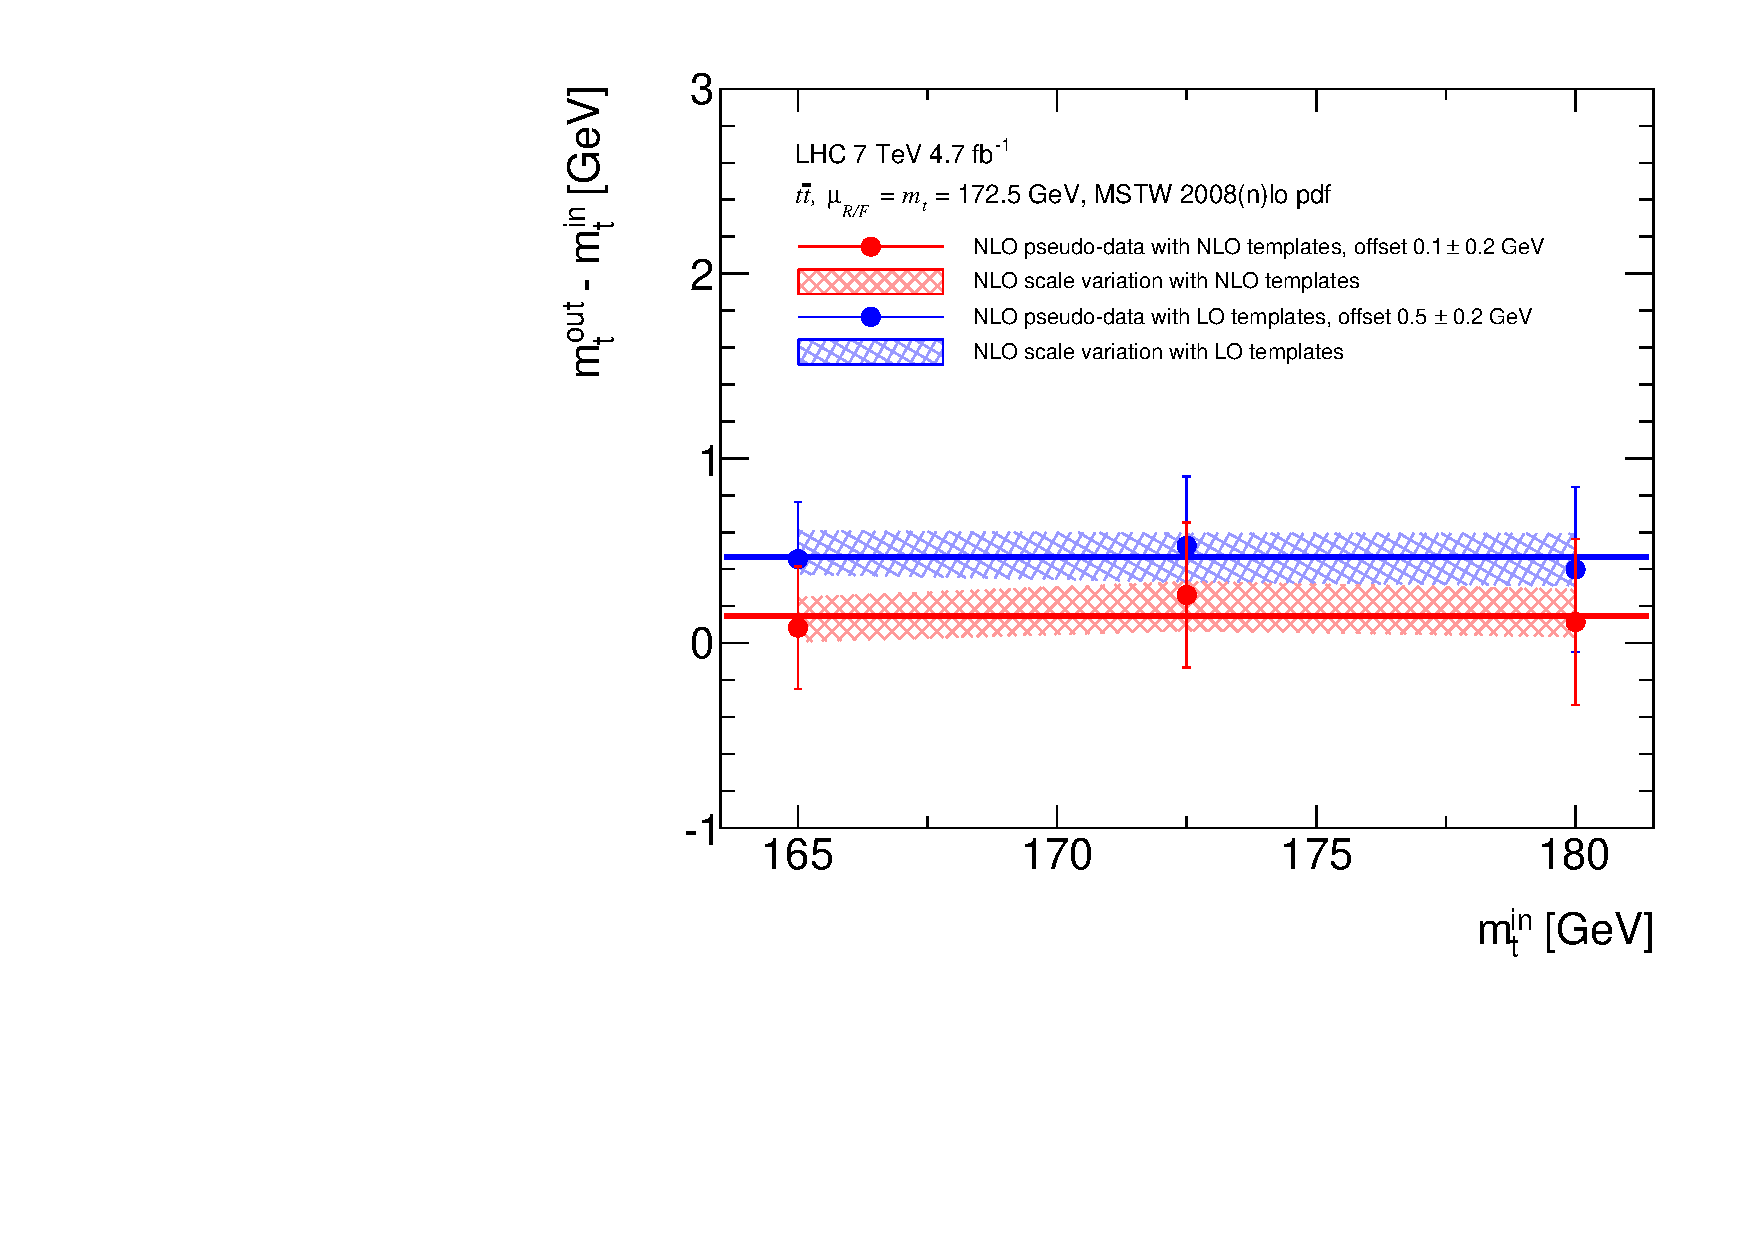
\includegraphics[width=0.49\textwidth]{./figs/fig10b.pdf}
  \label{sfig:effectstt}
}
\subfloat[Full]{
  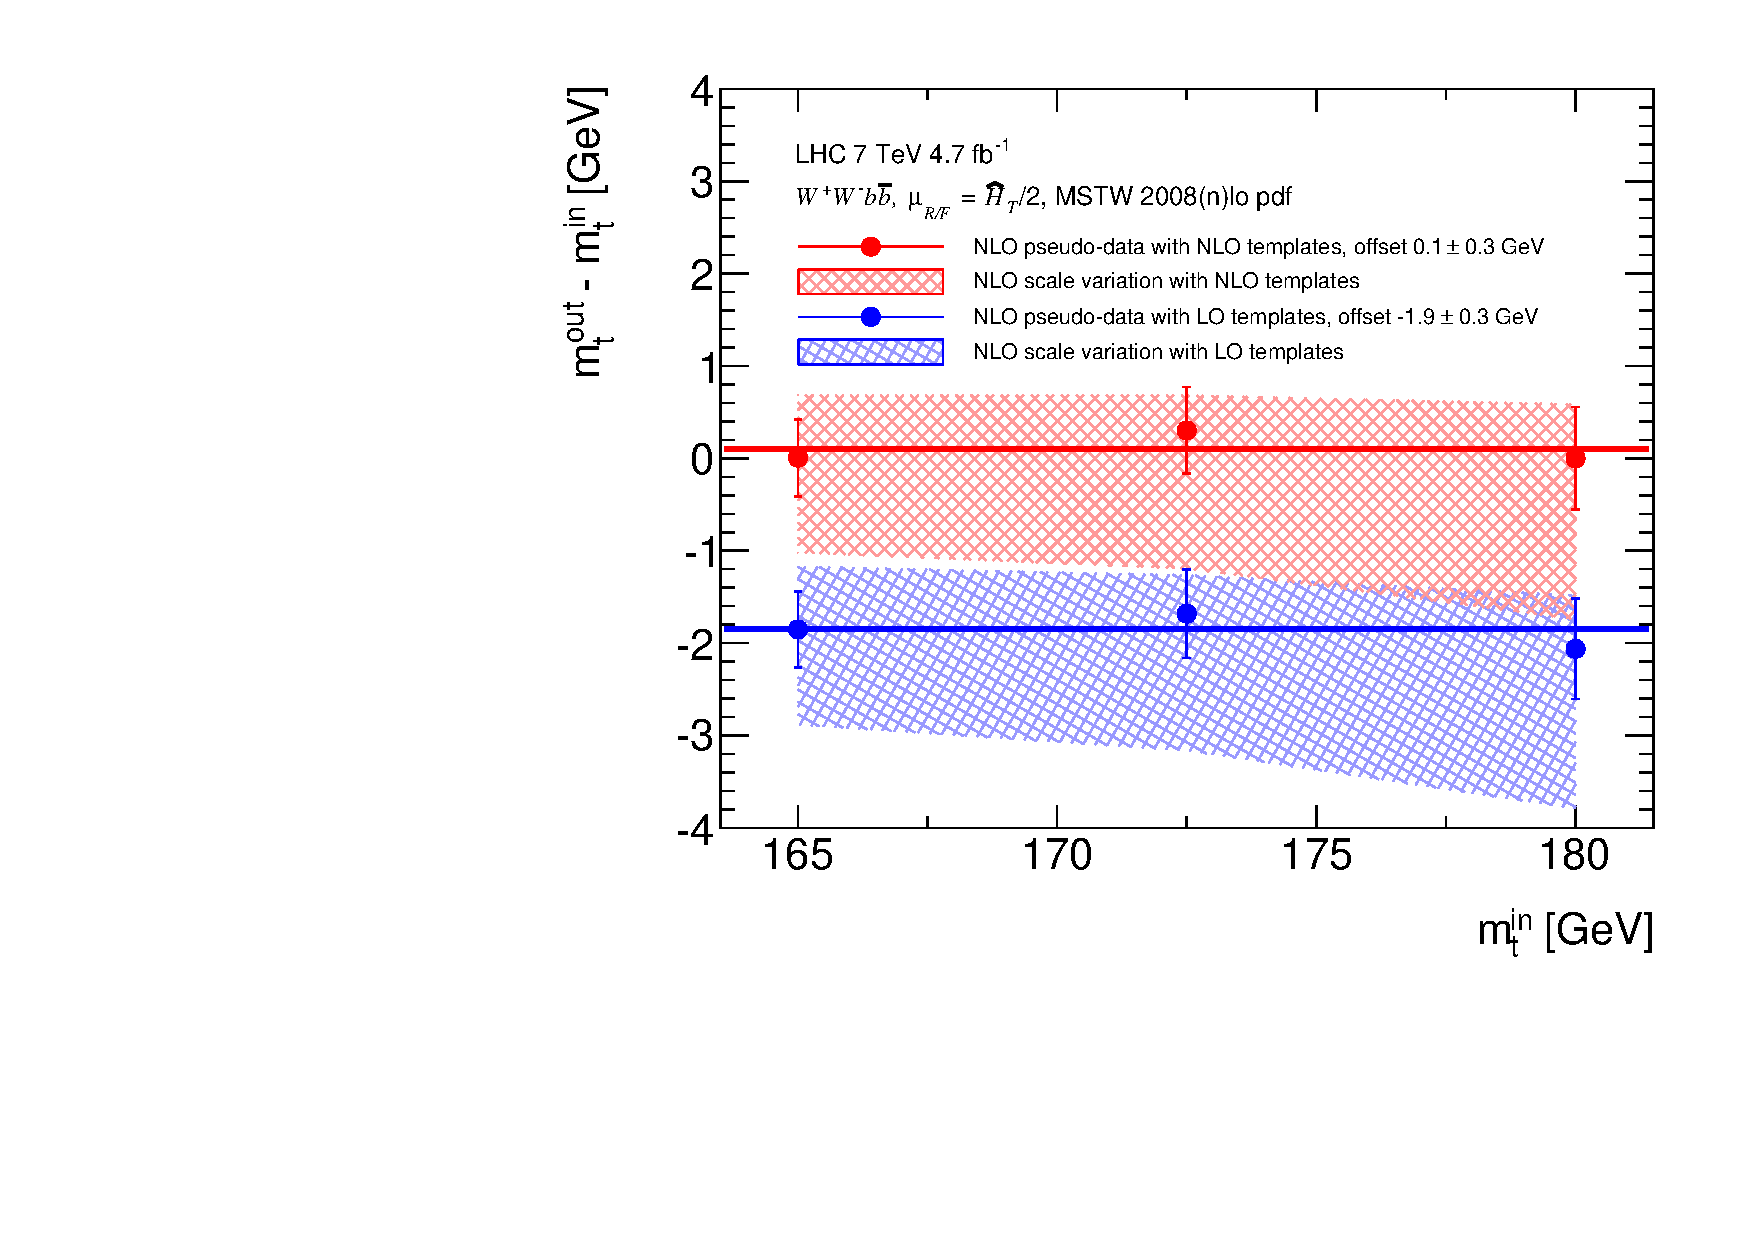
\includegraphics[width=0.49\textwidth]{./figs/fig9b.pdf}
  \label{sfig:effectsWWbb}
}
\caption[Quantitative effects of scale variations at \genlevel]{
%
An example pseudo-dataset (black dots) for $\intlumi=4.7~\invfb$ generated at \gls{NLO} in \subref{sfig:pseudott} the factorised and \subref{sfig:pseudoWWbb} the full approach. The corresponding template fit function (red line) and the underlying prediction (black histogram) are shown as well.
%
The observed mean residuals $\mtout-\mtin$ are given for the factorised approach in \fig~\subref{sfig:effectstt} and for the full approach in \fig~\subref{sfig:effectsWWbb} for three input mass values \mtin, using either \gls{LO} (blue) or \gls{NLO} templates (red). 
%
The uncertainty bars are statistical only, and the bands show the size of the respective scale variation. 
%
The result of a constant fit to the respective points is drawn as solid line.
%
The vertical axis ranges differ by a factor of 2.
%
}
%
\label{fig:NLOeffects}
\end{figure*}
%%%%%%%%%%%%%%%%%%%%%%%%%%%%%%%%%%%%%%%%%%%%%%%%%%%%%%%%%%%%%%%%%%%%%%%%%%%%%%%
%

The resulting \mt\ differences for the different scenarios are summarised in \fig~\subref*{sfig:effectstt} for the factorised and in \fig~\subref{sfig:effectsWWbb} for the full approach. These figures show the observed mass difference of the underlying and the resulting \tquark\ mass \mtin\ and \mtout, obtained as the average fit result from 1000 pseudo-experiments for input values $\mtin=165$, $172.5$ and $180$~\GeV. The $\mtout-\mtin$ residuals, corresponding to a consistent set of the \gls{NLO} pseudo-data and \gls{NLO} template fit function, are drawn in red, while the values using the \gls{LO} template fit functions for the fit to the \gls{NLO} pseudo-data are drawn in blue. The uncertainty bars are statistical and assigned to correspond to $\intlumi=4.7~\invfb$. A constant line has been fitted to each of the results to derive the average deviation. 
%
The compatibility of the red points with 0 demonstrates the internal consistency of the method, proving that it is unbiased. 
%
As expected from the shape differences visible in \fig~\ref{fig:mlbnlo}, the \mt\ deviations of the \gls{LO} to the \gls{NLO} template fit results for the factorised approach in \fig~\subref*{sfig:effectstt} amount to about $0.5$~\GeV\ and are low compared to the full approach in \fig~\subref*{sfig:effectsWWbb}, deviating by about $-1.9$~\GeV.
%
Consequently, provided the data follow the \gls{NLO} prediction, the usage of \gls{LO} templates in a \mt\ measurement at \recolevel\ would lead to a sizeable offset. 
%
The uncertainty bands in both figures correspond to the variation of the respective scale by a factor $2$ and $1/2$. This is applied to the \gls{NLO} pseudo-data, while leaving the templates unchanged. Due to the approximately linear behaviour of the template fit, the bands around the \gls{LO} and the \gls{NLO} values are very similar in size.
%
For the factorised approach, the symmetric uncertainty bands shown in \fig~\subref*{sfig:mlbnwa} result in a coherent shift across bins, resulting mostly in a change of normalisation, which does not affect the analysis. Therefore, the scale variation  only results in a mass difference of $\Delta \mt=\pm0.2~\GeV$. This is consistent in size with the experimental findings at \recolevel\ presented in \sect~\ref{sect:systtbarmod7TeV}. 
%
For the full approach, the corresponding uncertainty bands in \fig~\subref*{sfig:mlbfull} are asymmetric and their size is \mlb\ dependent. Consequently, the induced changes affect the shape of the \mlb\ distribution. The resulting mass difference is $\Delta \mt=^{+0.6}_{-1.0}~\GeV$, significantly larger than the factorised results. 
%
Given that the \gls{NWA} is an approximation of the full calculation, this hints at relevant effects from non-factorising contributions and higher-order corrections that are neglected when using the \gls{NWA} and \gls{LO} decays.
















\section{Summary}
%
The \gls{NLO} corrections to the process \ppWWbb\ have been calculated including non- and singly-resonant contributions. The results have been compared with the ones from a \gls{NLO} calculation in the \gls{NWA}, and quantified in terms of an induced expected difference in the measured \tquark\ mass at \genlevel. 
%
Besides the expected significant improvement in accuracy due to the additional order in \alphas, when compared to the corresponding \gls{LO} calculation, the inclusion of the non-factorising contributions has a sizeable impact on the shape of the estimator distribution \mlb. The scale variation uncertainty for the factorised calculation is found to be consistent with the one estimated at \recolevel, currently used in experimental measurements. The large effect at \genlevel\ using the full calculation hints at a possible underestimation of this uncertainty category for current measurements. 
%
These effects may or may not persist at \recolevel, where direct \mt\ measurements are performed and theoretical uncertainties are evaluated. 
%
It may also partly be covered by double-counting effects within the various modelling uncertainty categories considered in the experimental measurements, which are of $\order(1)$~\GeV\ for the $\sqrts=7$~\TeV\ measurement.
%
However, the final conclusion can only be drawn once a parton shower can be matched to the full \gls{NLO} calculation. The remaining difficulties are only of technical nature and a first successful matching has already been performed for single \tquark\ production, using a series of simplifications~\cite{Jezo:2015aia}. A definite answer on the transferability of the presented \genlevel\ results to \stablevel\ can therefore be expected in near future.
%
%Until then, the results can serve for the identification of observables and phase spaces, which are least susceptible to theoretical modelling uncertainties but still sensitive to the \tquark\ mass.